\subsection{Anzeigen aller Stationen}
\label{sub:anzeigen_aller_stationen}
  Nachdem zuvor alle Trips mit ihren Polylines in der Karte angezeigt wurden, folgt nun das Anzeigen aller Stationen, die zu einem Trip gehören. Ähnlich wie beim Abfragen und Anzeigen aller Polylines, sollte dieser Schritt mögliche Engpässe oder unvorhergesehene Probleme aufdecken (Abbildung \ref{fig:prozess/draw_all_stations}).

  \begin{figure}[htbp]
     \begin{center}
       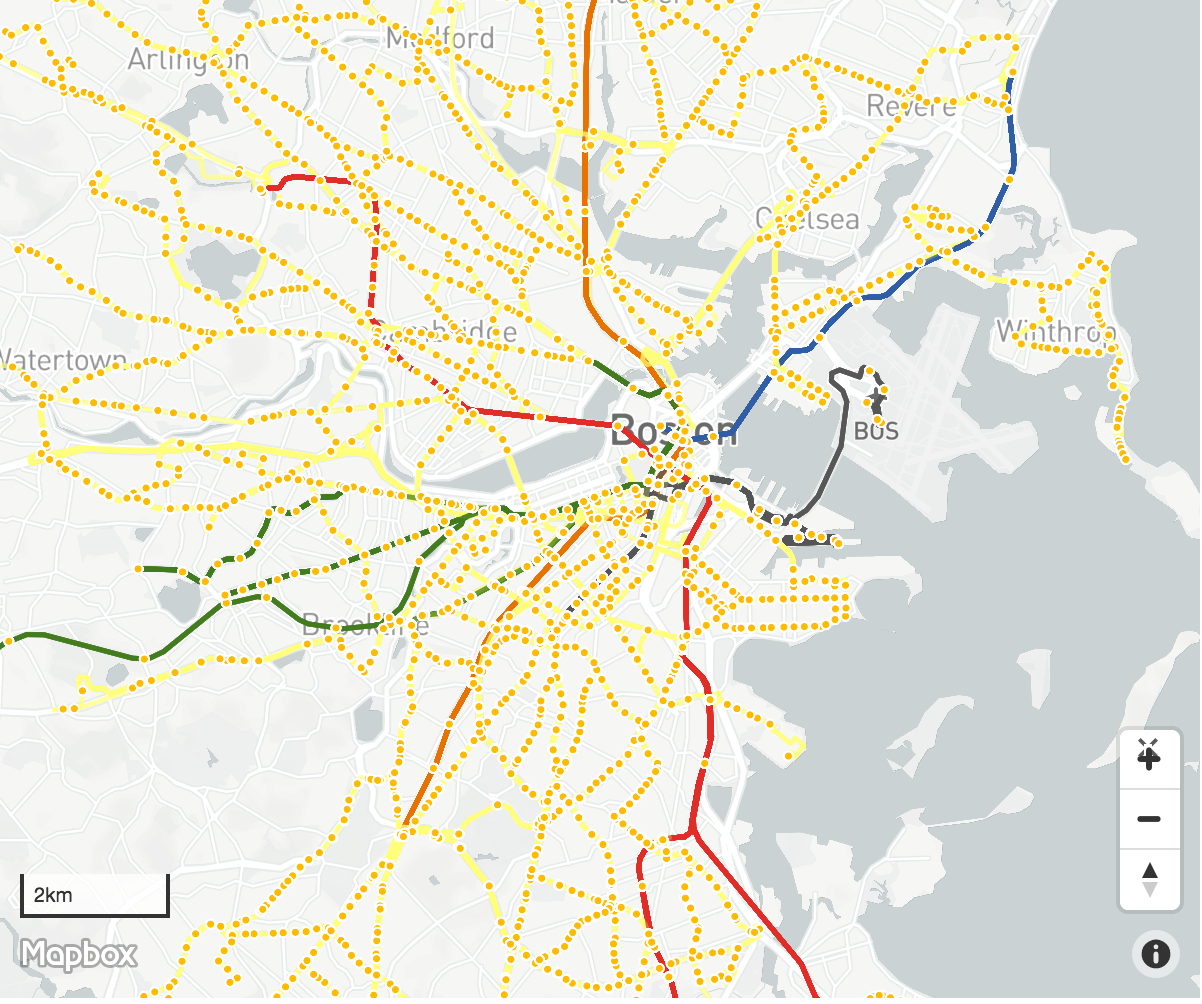
\includegraphics[width=0.6\textwidth]{prozess/draw_all_stations}
       \caption{Aktive Trips mit ihren dazugehörenden Stationen}
       \label{fig:prozess/draw_all_stations}
     \end{center}
   \end{figure}
   
  Vor allem die Abfrage von aktiven Trips aus der Datenbank, stellte ein großes Problem dar. Die Datenbank konnte die Anfragen des Clients nicht effizient genug verarbeiten. An dieser Stelle stand fest, dass für die weitere Arbeit umfassende Optimierungen der Datenbank erfolgen müssen, um eine responsive Webanwendung zu ermöglichen. 

  \subsubsection{GTFS Optimierungen}
  \label{ssub:gtfs_optimierungen}
    Durch eine Optimierung des GTFS Feeds lässt sich die Datenmenge bereits vor dem Importieren in die Datenbank erheblich verringern. Ein entsprechendes Tool hierfür ist \texttt{gtfstidy} \url{https://github.com/patrickbr/gtfstidy}. Es bietet allerdings nicht nur die Möglichkeit für die Vereinfachung von Polylines, sondern liefert eine ganze Reihe weiterer Optimierungsmöglichkeiten. 

    Der Kommandozeilenbefehl \colorbox{materialGrey}{\texttt{\color{white}{\$ gtfstidy -sSiRDeO input.zip output}}} optimiert das Stuttgart-VVS Feed wie folgt:
    
    \begin{itemize}[label={}]
      \item \textbf{-s} reduziert die Punktanzahl einer Polyline.
        
      \item \textbf{-S} entfernt redundante Polylines.

      \item \textbf{-i} wandelt Zeichen-ID's (String) in Zahlen-ID's (Integer).\footnote{Aus der String ID \texttt{'1.T0.10-1-j17-1.16.H'} wird \texttt{78}}

      \item \textbf{-O} entfernt Feed-Einträge, die nicht referenziert werden.

      \item \textbf{-R} entfernt doppelt vorhandene Routen.

      \item \textbf{-e} setzt fehlerhafte oder optionale Felder auf einen Standardwert.

      \item \textbf{-D} entfernt fehlerhafte Einträge aus dem Feed.
    \end{itemize}

    Durch Verwendung von gtfstidy konnte das Feed optimiert werden und die Datengröße der einzelnen Dateien um folgendes Maß verringert werden:

    \begin{longtable}{|>{\raggedright \arraybackslash}p{5.0cm}|>{\raggedright \arraybackslash}p{4.0cm}|>{\raggedright \arraybackslash}p{4.0cm}|}
      \hline
      Dateiname & Größe davor& Größe danach\\
      \hline
      {\small trips.txt}           & {\small 6 MB    } & {\small 2.8 MB  }\\
      {\small stop\_times.txt}     & {\small 103 MB  } & {\small 53 MB   }\\
      {\small stops.txt}           & {\small 651 KB  } & {\small 355 KB  }\\
      {\small shapes.txt}          & {\small 77.3 MB } & {\small 22.4 MB }\\
      {\small routes.txt}          & {\small 54 KB   } & {\small 38 KB   }\\
      {\small calendar\_dates.txt} & {\small 557 KB  } & {\small 463 KB  }\\
      \hline
      \caption{Tabellengröße bevor und nach anwenden von gtfstidy}
      \label{tbl:gtfs_tidy_results}
    \end{longtable}

    Insgesamt konnte so die Größe des Feeds von 79 MB auf 118 MB um knapp 50\% verringert werden. Vor allem die Umwandlung von langen String-ID's in kürzere Integer-ID's trägt maßgeblich zur Verringerung der Dateigröße bei.

  % subsubsection gtfs_optimierungen (end)

  \subsubsection{Denormalisierung der Datenbank}
  \label{ssub:denormalisierung_der_datenbank}
    Die Denormalisierung ist eine Strategie, die auf eine zuvor normalisierte Datenbank angewendet wird, um die Leistung zu erhöhen. Die Denormalisierung ist der Prozess, bei dem versucht wird, die Leseperformance einer Datenbank zu verbessern. Durch das Hinzufügen redundanter Kopien von Daten oder deren Gruppierung wird die Schreibleistung verringert.\parencite{sanders}
    Da die Daten ausschließlich ausgelesen und nicht geschrieben werden, ergeben sich nur Vorteile.\\

    Um diese Methode anwenden zu können, wird eine neue Tabelle generiert, die den Zugriff auf die benötigten Daten vereinfacht. Im Grunde handelt es sich um eine Vorberechnung. Anstatt die Tabellen bei jeder Anfrage an den Server aufwendig über viele \texttt{SQL-JOINS} zu verknüpfen, wird diese Verknüpfung einmalig vorberechnet und in einer Tabelle gespeichert. Die Denormalisierung  einer Tabelle wurde bereits im vorherigen Abschnitt "`\nameref{ssub:aggregieren_der_shape_tabelle}"' aufgezeigt. Dadurch ließ sich die Polyline über eine einzige Tabellenreihe abfragen, was die Performance signifikant erhöhte. Zum besseren Verständnis der Denormalisierungsmethode soll folgende Abbildung dienen:

    \begin{figure}[htbp]
      \begin{center}
        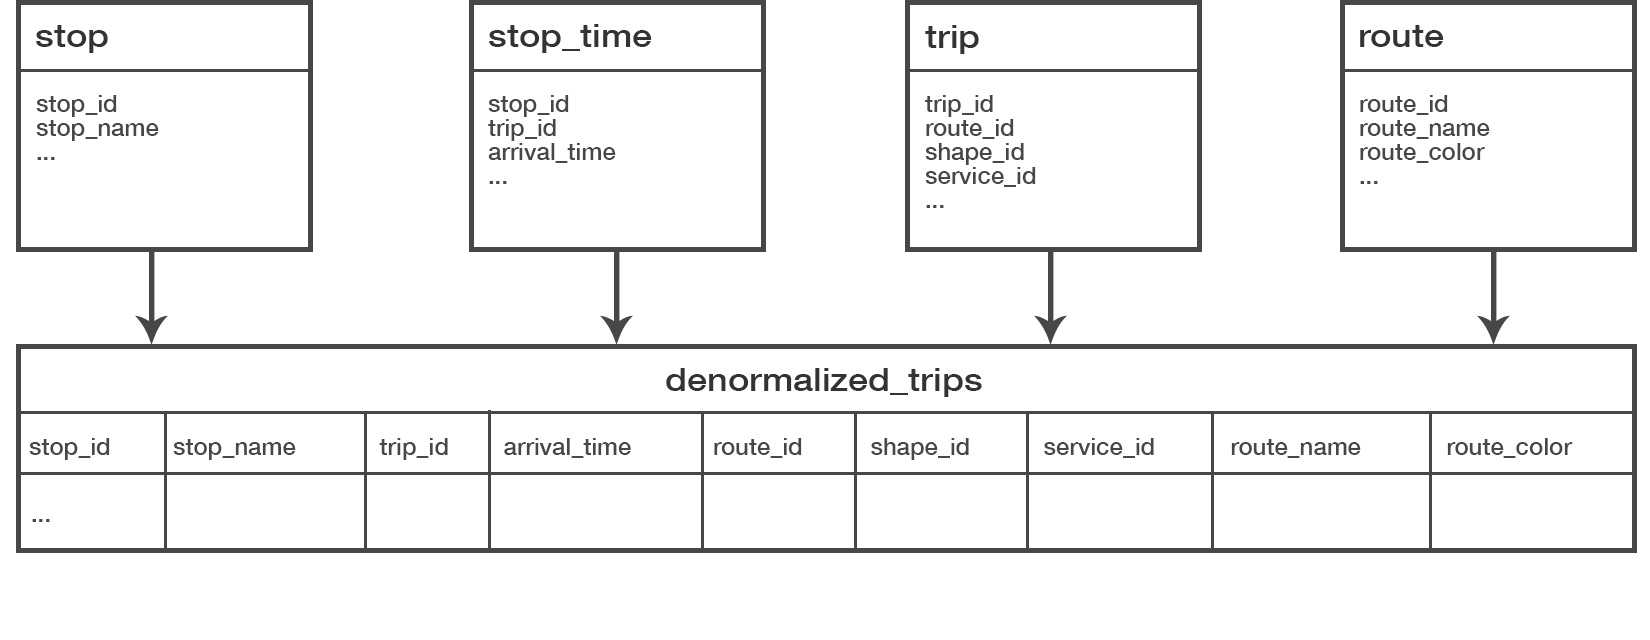
\includegraphics[width=\textwidth]{denormalizing.jpg}
        \caption{Beispiel einer Denormalisierung von Tabellen}
        \label{fig:denormalizing}
      \end{center}
    \end{figure}

    Abbildung \ref{fig:denormalizing} zeigt, wie aus einer vertikalen Anordnung eine horizontale Anordnung der einzelnen Datenfelder in einer einzigen \texttt{denormalized\_trips} Tabelle erzeugt wird. Eine Reihe in dieser neuen Tabelle steht für genau einen Eintrag eines Trips. Anstatt also bei jeder Anfrage an den Server die verschiedenen Daten mittels \texttt{JOIN} verknüpfen zu müssen, können diese jetzt per Zugriff auf eine einzige Reihe in nur einer Tabelle abgefragt werden.

    Dieses Prinzip der Gruppierung von Daten in einer neuen Tabelle soll nun auch auf die anderen benötigten Tabellen angewendet werden. Die Denormalisierung erfolgt in 3 Schritten:

    \begin{enumerate}
      \item Erstellen der neuen Tabelle \texttt{denormalized\_trips}
      \item Importieren der verschiedenen Daten in diese neue Tabelle
      \item Abfragen der Datenn über diese neue Tabelle
    \end{enumerate}

    Das SQL-Statement ist abermals aufgrund seiner Länge dem Anhang \ref{lst:denormalized_shapes} zu entnehmen. Dargestellt in einer Tabelle, sieht das SQL-Statement wie folgt aus:

    \begin{figure}[htbp]
      \begin{center}
        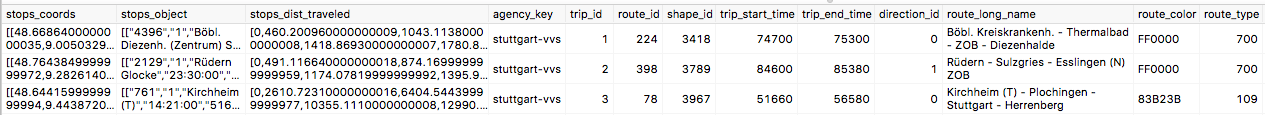
\includegraphics[width=\textwidth]{denormalized_tables.png}
        \caption{Auszug aus der \texttt{denormalized\_trips} Tabelle}
        \label{fig:denormalized_table}
      \end{center}
    \end{figure}  

    \subsubsection*{Ergebnisse der Denormalisierung}
    \label{ssub:ergebnisse_der_denormalisierung}
      Für die Visualisierung ist eine Abfrage der aktiven Trips am wichtigsten, da diese die Daten für die Darstellung der Vehicle auf der Karte liefert. Wie in Abbildung \ref{fig:denormalizing_results} zu sehen ist, wird auf die \texttt{denormalized\_trips}, \texttt{denormalized\_shapes} und die \texttt{calendar\_dates} Tabelle zugegriffen. Dabei werden die einzelnen Tabellen über die \texttt{shape\_id} und \texttt{service\_id} miteinander verknüpft. Das Resultat ist die Ausgabe aller aktiven Trips in einem variabel definierbarem Zeitraum des aktuellen Datums.

      \begin{figure}[htbp]
        \begin{center}
          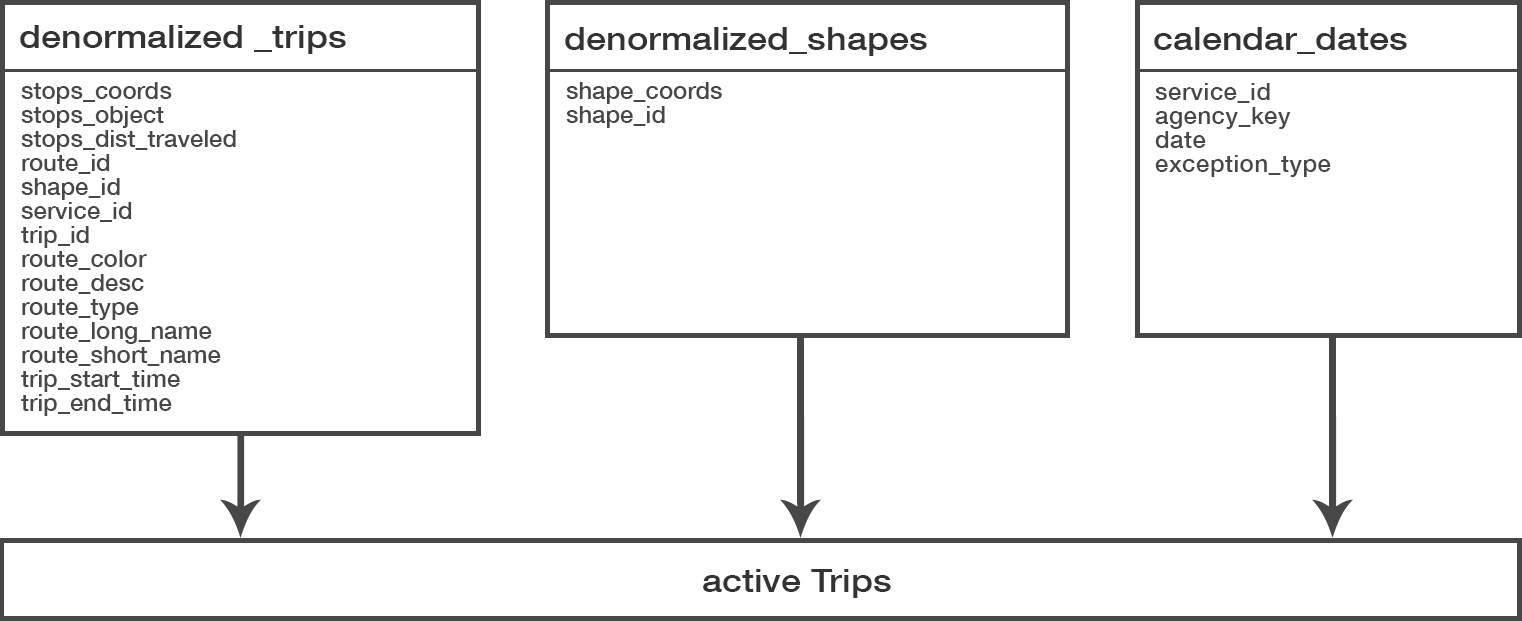
\includegraphics[width=\textwidth]{denormalizing_results.jpg}
          \caption{Benötigte Tabellen zur Abfrage von Trips}
          \label{fig:denormalizing_results}
        \end{center}
      \end{figure} 

      Nachfolgend werden in Tabelle \ref{tbl:evaluierung_der_denormalisierung} die Ergebnisse der Evaluation für die Abfrage der aktiven Trips in einem wachsenden Zeitraum dargestellt. Die verwendete SQL-Abfrage befindet sich im \nameref{sec:anhang} unter Listing \ref{lst:query_trips}.

      \begin{longtable}{|>{\raggedright \arraybackslash}p{5.0cm}|>{\raggedright \arraybackslash}p{5.0cm}|>{\raggedright \arraybackslash}p{4.0cm}|}
      \caption{Evaluierung der Denormalisierung}\label{tbl:evaluierung_der_denormalisierung}\\
        \hline
          Zeitraum & Trip Anzahl & Query Zeit\\
        \hline
          {\small 9:00 bis 9:15} & {\small 88} & {\small 98 ms}\\
          {\small 9:00 bis 10:00} & {\small 1125} & {\small 154 ms}\\
          {\small 9:00 bis 12:00} & {\small 3360} & {\small 285 ms}\\
          {\small 9:00 bis 15:00} & {\small 7070} & {\small 497 ms}\\
          {\small 9:00 bis 21:00} & {\small 14718} & {\small 900 ms}\\
        \hline
      \end{longtable}

      Die Ergebnisse zeigen, dass die Abfragezeit der Datenbank für die aktiven Trips erheblich gesunken ist. Zu Projektbeginn war eine solch effiziente Abfrage aufgrund der überaus langen Laufzeit ($> 1min$) nicht möglich.

      \begin{figure}[htbp]
        \begin{center}
          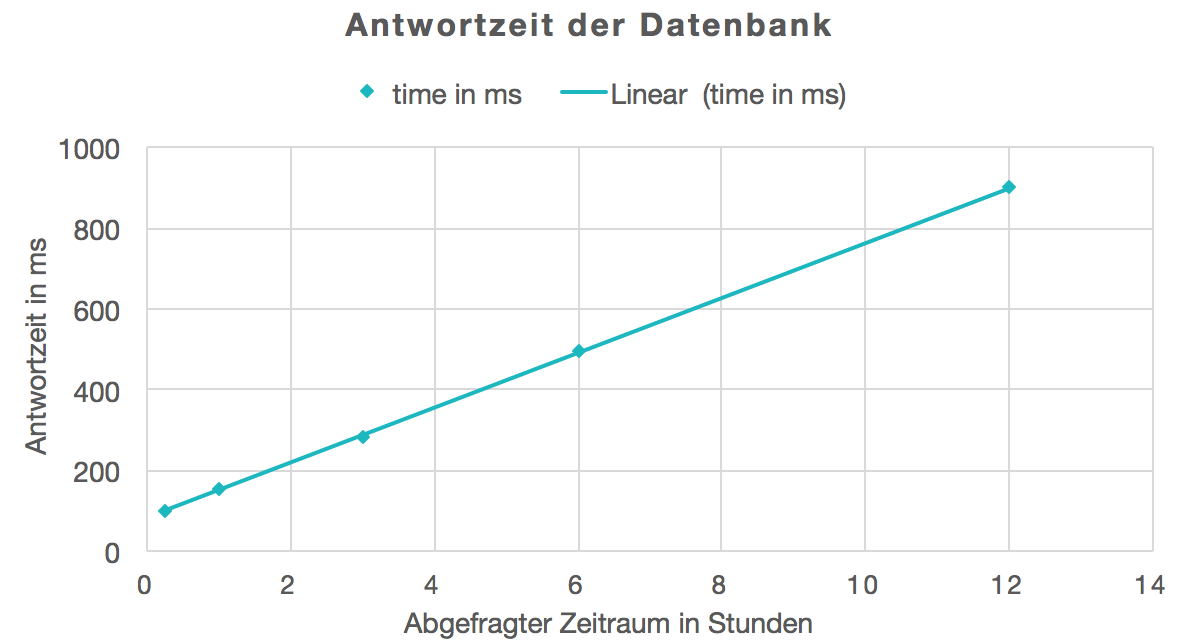
\includegraphics[width=0.7\textwidth]{query_time_chart}
          \caption{Plot der Abfragezeiten}
          \label{fig:query_time_chart}
        \end{center}
      \end{figure}

      \pagebreak
      
      Abbildung \ref{fig:query_time_chart} zeigt einen Plot der Query-Zeit aus Tabelle \ref{tbl:evaluierung_der_denormalisierung} als linearen Graphen. Daraus ist ersichtlich, dass die Antwortzeit der Datenbank linear mit dem abgefragten Zeitraum wächst. Für die Visualisierung sind vor allem zwei Abfragen wichtig: Erstens das Abfragen eines größeren Zeitraums von 1-2 Stunden. Dies geschieht beim ersten Aufrufen der Webanwendung wenn die Karte noch keine Trips besitzt und damit leer ist. Zweitens die Abfrage von kleinen Zeiträumen von nur einer Minute, um neue Trips abzufragen. Für diese zwei Abfragen bewegt sich die Antwortzeit des Servers zwischen $\approx 80 -  160\; ms$. Damit wurde das in Kapitel \ref{sub:zielsetzung} gesetzte Ziel von 0 bis $200ms$ bereits erreicht.
      
    % subsubsection ssub:ergebnisse_der_denormalisierung (end)
  % subsubsection denormalisierung_der_datenbank (end)
% subsection anzeigen_aller_stationen (end)